\chapter{Αλγόριθμος Black-Scholes}
\label{chap:black_scholes}

\section{Εισαγωγή}
\begin{itemize}
  \item Ο αλγόριθμος Black-Scholes είναι ένα μοντέλο για την τιμολόγηση ευρωπαϊκών δικαιωμάτων προαίρεσης.
  \item Ο αλγόριθμος αυτός αναπτύχθηκε το 1973 από τους Fischer Black, Myron Scholes και Robert Merton.
  \item Η εξίσωση Black-Scholes είναι μια διαφορική εξίσωση που περιγράφει την εξέλιξη της τιμής ενός δικαιώματος προαίρεσης με την πάροδο του χρόνου.
\end{itemize}

Σημαντικότητα
  \begin{itemize}
    \item Ο αλγόριθμος Black-Scholes έχει επηρεάσει σημαντικά την ανάπτυξη των χρηματοοικονομικών αγορών.
    \item Έχει κερδίσει το βραβείο Νόμπελ Οικονομίας το 1997 για την εφαρμογή του στη χρηματοοικονομική θεωρία.
  \end{itemize}

\section{Παλαιότερες Μέθοδοι}

Πριν την ανάπτυξη του μοντέλου Black-Scholes, η αποτίμηση των δικαιωμάτων προαίρεσης βασιζόταν κυρίως στην έννοια της \textbf{εγγενούς αξίας} (\textit{intrinsic value}).
Η εγγενής αξία ενός δικαιώματος προαίρεσης ορίζοταν ως η διαφορά μεταξύ της τρέχουσας τιμής της μετοχής και της τιμής άσκησης του δικαιώματος (\(S_0 - X\)), εφόσον αυτή είναι θετική. Εάν η τιμή άσκησης είναι ίση με την τρέχουσα τιμή της μετοχής, τότε η εγγενής αξία είναι μηδέν.
Ωστόσο, ένα δικαίωμα προαίρεσης με μηδενική εγγενή αξία κατά την ημερομηνία χορήγησης δεν σημαίνει ότι δεν έχει καμία αξία συνολικά. Υπάρχει πάντα η πιθανότητα η τιμή της μετοχής να αυξηθεί στο μέλλον, προσφέροντας στον κάτοχο του δικαιώματος τη δυνατότητα να αγοράσει τη μετοχή σε χαμηλότερη τιμή από την τρέχουσα τιμή της αγοράς. Αυτή η πιθανότητα δημιουργεί την \textbf{χρονική αξία} (\textit{time value}) του δικαιώματος προαίρεσης.
Η χρονική αξία αντικατοπτρίζει το ενδεχόμενο μελλοντικής κερδοφορίας λόγω της μεταβλητότητας της αγοράς και του χρόνου που απομένει μέχρι τη λήξη του δικαιώματος. Όσο μεγαλύτερη είναι η μεταβλητότητα της μετοχής ή ο χρόνος μέχρι τη λήξη, τόσο μεγαλύτερη είναι η χρονική αξία του δικαιώματος. Έτσι, ακόμη και όταν η εγγενής αξία είναι μηδενική, το δικαίωμα προαίρεσης διατηρεί αξία λόγω της πιθανότητας ευνοϊκών μεταβολών στην τιμή της μετοχής.
Η κατανόηση αυτής της διαφοράς μεταξύ εγγενούς και χρονικής αξίας ήταν καθοριστική για την ανάπτυξη πιο σύνθετων και ακριβών μοντέλων αποτίμησης, όπως το μοντέλο Black-Scholes, το οποίο λαμβάνει υπόψη τόσο την εγγενή όσο και τη χρονική αξία ενός δικαιώματος προαίρεσης.

Το μοντέλο Black-Scholes ήταν το πρώτο ευρέως χρησιμοποιούμενο μοντέλο αποτίμησης δικαιωμάτων προαίρεσης που έλαβε υπόψη το 
στοιχείο της χρονικής αξίας μαζί με την εγγενή αξία. Η χρονική αξία είναι η αξία που υπάρχει κατά τη χρονική περίοδο στην οποία το δικαίωμα προαίρεσης
μπορεί να ασκηθεί, σε σχέση με το ενδεχόμενο κέρδους από τόκους και την πιθανή αύξηση της τιμής της μετοχής (μεταβλητότητα).

\subsection{Παράδειγμα: Επεξήγηση της Χρονικής Αξίας με Πράξεις}

Έστω ένα δικαίωμα προαίρεσης αγοράς (call option) με διάρκεια ζωής 10 έτη και τιμή άσκησης X = \$5. Την ημερομηνία χορήγησης, η τιμή της μετοχής $S_0$ είναι επίσης \$5. 
Παρόλο που η εγγενής αξία είναι μηδενική, το δικαίωμα προαίρεσης έχει χρονική αξία, επειδή ο κάτοχος έχει τη δυνατότητα να επωφεληθεί από πιθανή αύξηση της τιμής της μετοχής
κατά τη διάρκεια των 10 ετών. 

Εγγενής Αξία = $\max(S_0 - X, 0) = \max(\$5 - \$5, 0) = \$0$

Η χρονική αξία εξαρτάται από παράγοντες όπως η μεταβλητότητα της τιμής της μετοχής και ο χρόνος μέχρι τη λήξη.
Όσο μεγαλύτερη είναι η μεταβλητότητα ή ο χρόνος μέχρι τη λήξη, τόσο μεγαλύτερη είναι η χρονική αξία, καθώς αυξάνεται η πιθανότητα η τιμή της μετοχής να ξεπεράσει την τιμή άσκησης.
Για να κατανοήσουμε τη χρονική αξία, ας εξετάσουμε το εξής σενάριο: ο κάτοχος αγοράζει το δικαίωμα προαίρεσης στην αγορά,
πληρώνοντας ένα ασφάλιστρο (option premium), το οποίο περιλαμβάνει τη χρονική αξία (καθώς η εγγενής αξία είναι μηδενική). Ας υποθέσουμε ότι το ασφάλιστρο είναι \$1 (ένα υποθετικό ποσό για απλότητα).
Μετά από 10 χρόνια, κατά τη λήξη του δικαιώματος, ισχύουν τα εξής:
\begin{itemize}
    \item Η τιμή της μετοχής είναι \$8 (αύξηση της τιμής της μετοχής).
    \item Κέρδος από την πώληση του δικαιώματος = $S_{10}$ - X - ασφάλιστρο = \$8 - \$5 - \$1 = + \$2
\end{itemize}

 test
Αν απο την άλλη πλευρά η τιμή της μετοχής είναι <= \$5, τότε:
\begin{itemize}
    \item Ο κάτοχος θα αποφασήσει να μην ασκήσει το δικαίωμα προαίρεσης, καθώς η τιμή της μετοχής είναι χαμηλότερη από την τιμή άσκησης.
    \item Οπότε μένει μόνο με ζημία το αρχικό κόστος του ασφαλίστρου Ζημία = ασφάλιστρο = \$1
\end{itemize}

Η χρονική αξία προκύπτει από τη δυνατότητα του κατόχου να επωφεληθεί από πιθανή άνοδο της τιμής της μετοχής χωρίς να δεσμεύσει το πλήρες ποσό της επένδυσης στην αγορά της μετοχής.
Αντί να αγοράσει τη μετοχή στα \$5, ο κάτοχος πληρώνει μόνο το ασφάλιστρο (\$1) για το δικαίωμα προαίρεσης, διατηρώντας έτσι το κεφάλαιο για άλλες επενδύσεις. (π.χ. σε ένα ομόλογο χωρίς κίνδυνο)
Για παράδειγμα, αν ο κάτοχος επενδύσει το υπόλοιπο ποσό (\$4) σε ένα ομόλογο με επιτόκιο 5\% για 10 χρόνια, θα έχει:
\begin{itemize}
    \item Μελλοντική αξία \( = \$4 \times (1 + 0.05)^{10} = \$4 \times 1.62889 = \$6.51557 \)
\end{itemize}

Αυτό σημαίνει ότι ο κάτοχος του δικαιώματος προαίρεσης έχει τη δυνατότητα να επωφεληθεί από την αύξηση της τιμής της μετοχής, διατηρώντας παράλληλα τη δυνατότητα επένδυσης σε άλλες ευκαιρίες
ενώ και στην περίπτωση που η τιμή της μετοχής δεν αυξηθεί, παραμένει ένα κέρδος.

\section{Αλγόριθμος Black Scholes}

H εξίσωση του μοντέλου θεωρεί ότι μέσα όπως μετοχές ή συμβόλαια μελλοντικής εκπλήρωσης:
\begin{itemize}
    \item θα έχουν μια λογαριθμοκανονική κατανομή των τιμών
    \item θα ακολουθεί έναν τυχαίο περίπατο με σταθερή μετατόπιση και μεταβλητότητα.
\end{itemize}

Η εξίσωση χρησιμοποιεί αυτή την υπόθεση και συνυπολογίζει άλλες σημαντικές μεταβλητές για να προκύψει η τιμή ενός δικαιώματος αγοράς ευρωπαϊκού τύπου.

Το μοντέλο Black-Scholes απαιτεί τις πέντε μεταβλητές που αναλύθηκαν προηγουμένως:
\begin{itemize}
    \item την τιμή άσκησης ενός δικαιώματος προαίρεσης
    \item την τρέχουσα τιμή της μετοχής
    \item το χρόνο μέχρι τη λήξη
    \item το επιτόκιο χωρίς κίνδυνο
    \item και τη μεταβλητότητα.
\end{itemize}

Επίσης περεταίρω παραδοχές που πρέπει να αναφερθούν είναι:

\begin{itemize}
    \item Η τιμή του υποκείμενου περιουσιακού στοιχείου ακολουθεί γεωμετρική κίνηση Brownian (αλλιως διαδικασία Wiener) η οποία περιγράφεται απο την εξίσωση:
    \begin{equation}
      dS = \mu S\,dt + \sigma S\,dW
    \end{equation}
    Οπου $W$ είναι μια τυχαία μεταβλητή που ακολουθεί κανονική κατανομή.
    Εχει μέση τιμή 0 και διασπορά $\sigma^2t$.
    \begin{figure}[H]
      \centering
      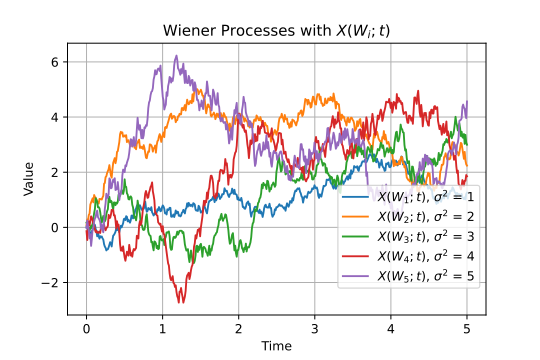
\includegraphics[width=1.0\textwidth]{./figures/chapter2/wiener_process.png}
      \caption{Γραφική απεικόνιση της γεωμετρικής κίνησης Brownian}
      \label{fig:black_scholes_brownian}
    \end{figure}
    \item Κατά τη διάρκεια της διάρκειας του δικαιώματος προαίρεσης δεν καταβάλλονται μερίσματα.
    \item Οι αγορές είναι τυχαίες επειδή οι κινήσεις της αγοράς δεν μπορούν να προβλεφθούν.
    \item Δεν υπάρχουν έξοδα συναλλαγής κατά την αγορά του δικαιώματος προαίρεσης.
    \item Το επιτόκιο χωρίς κίνδυνο και η μεταβλητότητα του υποκείμενου περιουσιακού στοιχείου είναι γνωστά και σταθερά.
    \begin{tcolorbox}[colframe=blue!50!black, colback=blue!5, title=Ορισμός Προαιρεσης Μετοχών]
        Η μεταβλητότητα στην πραγματικότητα δέν ειναι σταθερή και είναι συνάρητηση του χρόνου μέχρι την λήξη και την τιμή  του δικαιώματος προαίρεσης.
        \begin{figure}[H]
          \centering
          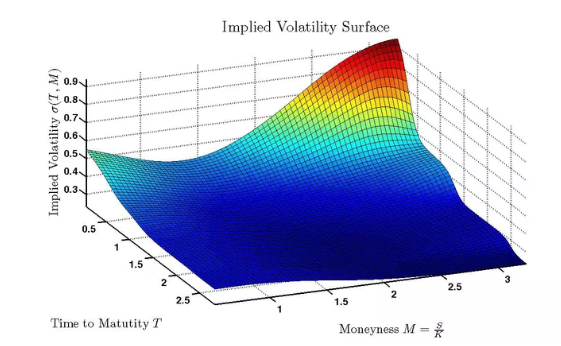
\includegraphics[width=1.0\textwidth]{./figures/chapter2/volatility_surface.png}
          \caption{Τρισδιάστατη απεικόνιση της επιφάνειας μεταβλητότητας}
          \label{fig:volatility_surface}
        \end{figure}
        Τα κύρια χαρακτηριστικά της επιφάνειας μεταβλητότητας είναι ότι τα δικαιώματα προαίρεσης με χαμηλότερες τιμές άσκησης τείνουν 
        να έχουν υψηλότερες μεταβλητότητες. Για μια δεδομένη λήξη $T$, αυτό το χαρακτηριστικό αναφέρεται συνήθως ως "volatility skew" ή "volatility smile".
        Για μια δεδομένη τιμή άσκησης $K$, η μεταβλητότητα μπορεί είτε να αυξάνεται είτε να μειώνεται με τον χρόνο μέχρι τη λήξη.
        Σε γενικές γραμμές, όμως, η $\sigma(K, T)$ τείνει να συγκλίνει σε μια σταθερά καθώς ο χρόνος μέχρι την λήξη τείνει στο άπειρο $T \to \infty$. 
        Για μικρές τιμές $T$, ωστόσο, συχνά παρατηρούμε μια αντεστραμμένη επιφάνεια μεταβλητότητας, με τα δικαιώματα προαίρεσης βραχυπρόθεσμης 
        λήξης να έχουν πολύ υψηλότερες μεταβλητότητες από τα μακροπρόθεσμα.
    \end{tcolorbox}
    \item Οι αποδόσεις του υποκείμενου περιουσιακού στοιχείου κατανέμονται κανονικά.
    \item Το δικαίωμα προαίρεσης είναι ευρωπαϊκό και μπορεί να ασκηθεί μόνο κατά τη λήξη.
\end{itemize}

Ο τύπος του Black-Scholes υπολογίζεται πολλαπλασιάζοντας την τιμή της μετοχής με τη συνάρτηση τυπικής κατανομής πιθανοτήτων. 
Η καθαρή παρούσα αξία (ΚΠΑ) της τιμής εξάσκησης πολλαπλασιαζόμενη με τη συσωρευτική τυπική κανονική κατανομή και αφαιρείται στη συνέχεια από την προκύπτουσα τιμή του προηγούμενου υπολογισμού.
Συμφωνα και με την βιβλιογραφία [\cite{wikipedia_black_scholes}, \cite{haugh_black_scholes_columbia}]:

\begin{equation}
    C = S_0 N(d_1) - X e^{-rT} N(d_2)
\end{equation}

όπου:
\begin{itemize}
    \item $C$: Η τιμή του δικαιώματος προαίρεσης
    \item $S_0$: Η τρέχουσα τιμή της μετοχής
    \item $X$: Η τιμή άσκησης του δικαιώματος προαίρεσης
    \item $r$: Το επιτόκιο χωρίς κίνδυνο
    \item $T$: Ο χρόνος μέχρι τη λήξη
    \item $N(d)$: Η συνάρτηση κατανομής κανονικής πιθανότητας
\end{itemize}

Τα $d_1$ και $d_2$ υπολογίζονται με τους παρακάτω τύπους:
\begin{equation}
    d_1 = \frac{\ln(\frac{S_0}{X}) + (r + \frac{\sigma^2}{2})T}{\sigma \sqrt{T}}
\end{equation}
\begin{equation}
    d_2 = d_1 - \sigma \sqrt{T}
\end{equation}

και το N(d) είναι η συνάρτηση κατανομής κανονικής πιθανότητας, που υπολογίζεται με τον παρακάτω τύπο:
\begin{equation}
    N(d) = \frac{1}{\sqrt{2\pi}} \int_{-\infty}^{d} e^{-\frac{x^2}{2}} dx
\end{equation}

Το πρώτο μισο της εξίσωσης δηλαδή το $S_0 N(d_1)$ είναι η εκτίμηση της τιμής ασκησης,
ενώ το δεύτερο μισό της εξίσωσης, $X e^{-rT} N(d_2)$, είναι η εκτίμηση της καθαρής παρούσας αξίας της τιμής άσκησης του δικαιώματος προαίρεσης.

\subsection{Σημασία της Θεωρίας}
Το μοντέλο Black-Scholes κατέχει μεγάλη σημασία στον οικονομικό χώρο διότι εισήγαγε μια αυστηρή μαθηματική προσέγγιση για την τιμολόγηση των δικαιωμάτων προαίρεσης,
επιτρέποντας στους επενδυτές και στους διαχειριστές κινδύνου να εκτιμήσουν με ακρίβεια την αξία αυτών των χρηματοοικονομικών εργαλείων.
Πριν από την ανάπτυξή του, η τιμολόγηση των options βασιζόταν κυρίως σε εμπειρικές μεθόδους ή σε υποκειμενικές εκτιμήσεις.

Η επαναστατικότητα του μοντέλου έγκειται στα εξής:
\begin{itemize}
    \item \textbf{Αυστηρή Θεωρητική Βάση:} Το μοντέλο βασίζεται σε θεμελιώδεις αρχές των μαθηματικών και της στατιστικής, όπως η κανονική κατανομή και η στοχαστική ανάλυση.
    \item \textbf{Απλοποίηση της Τιμολόγησης:} Παρέχει έναν απλό και πρακτικό τύπο για την τιμολόγηση των ευρωπαϊκών δικαιωμάτων προαίρεσης, μειώνοντας την πολυπλοκότητα της διαδικασίας.
    \item \textbf{Ενίσχυση της Αγοράς Παραγώγων:} Η εφαρμογή του μοντέλου συνέβαλε στην ανάπτυξη και την ωρίμανση της αγοράς παραγώγων, καθιστώντας την πιο διαφανή και αποτελεσματική.
    \item \textbf{Διαχείριση Κινδύνου:} Το μοντέλο επιτρέπει στους επενδυτές να αντισταθμίσουν κινδύνους (hedging) με μεγαλύτερη ακρίβεια, βελτιώνοντας τη στρατηγική τους.
    \item \textbf{Επιστημονική Αναγνώριση:} Η απονομή του Βραβείου Νόμπελ στους δημιουργούς του υπογραμμίζει τη σημασία του για τη χρηματοοικονομική επιστήμη.
\end{itemize}

Η εισαγωγή του μοντέλου Black-Scholes άλλαξε ριζικά τον τρόπο με τον οποίο οι αγορές αντιλαμβάνονται και διαχειρίζονται τα δικαιώματα προαίρεσης, καθιστώντας το ένα από τα πιο σημαντικά επιτεύγματα στη χρηματοοικονομική μηχανική.

\section{Εφαρμογές}

Ο αλγόριθμος Black-Scholes έχει ευρεία εφαρμογή στον χρηματοοικονομικό τομέα και αποτελεί τη βάση για πολλές σύγχρονες στρατηγικές επένδυσης και διαχείρισης κινδύνου.

\subsection{Τιμολόγηση Δικαιωμάτων Προαίρεσης}

\begin{itemize}
  \item \textbf{Ευρωπαϊκά δικαιώματα προαίρεσης:} Το κύριο πεδίο εφαρμογής του μοντέλου, όπου το δικαίωμα μπορεί να ασκηθεί μόνο κατά τη λήξη.
  \item \textbf{Αμερικανικά δικαιώματα προαίρεσης:} Τροποποιημένες εκδόσεις του μοντέλου για δικαιώματα που μπορούν να ασκηθούν ανά πάσα στιγμή μέχρι τη λήξη.
  \item \textbf{Δικαιώματα προαίρεσης σε μετοχές και δείκτες:} Εφαρμογή σε διάφορα υποκείμενα περιουσιακά στοιχεία.
  \item \textbf{Exotic Options:} Βάση για την ανάπτυξη πιο σύνθετων δικαιωμάτων προαίρεσης με ειδικά χαρακτηριστικά.
\end{itemize}

\subsection{Διαχείριση Κινδύνου και Hedging}

\begin{itemize}
  \item \textbf{Delta Hedging:} Χρήση του δέλτα για τη δημιουργία ουδέτερων θέσεων ως προς τις μεταβολές της τιμής.
  \item \textbf{Gamma Hedging:} Προστασία έναντι μεταβολών.
  \item \textbf{Vega Hedging:} Διαχείριση του κινδύνου μεταβλητότητας.
  \item \textbf{Βελτιστοποίηση χαρτοφυλακίου:} Βελτιστοποίηση χαρτοφυλακίων με χρήση παραγώγων.
\end{itemize}

\subsection{Εταιρικές Εφαρμογές}

\begin{itemize}
  \item \textbf{Μοίρασμα εταιρικών δικαιωμάτων:} Αποτίμηση δικαιωμάτων προαίρεσης εργαζομένων.
  \item \textbf{Αποτίμηση:} Αποτίμηση επενδυτικών ευκαιριών και στρατηγικών επιλογών.
  \item \textbf{Πιστωτικός Έλεγχος:} Εφαρμογή σε μοντέλα πιστωτικού κινδύνου.
\end{itemize}

\subsection{Αλγοριθμική Διαπραγμάτευση}

\section{Περιορισμοί και Προκλήσεις}

\subsection{Θεωρητικοί Περιορισμοί}

\begin{itemize}
  \item \textbf{Υπόθεση Σταθερής Μεταβλητότητας:} Στην πραγματικότητα, η μεταβλητότητα αλλάζει διαρκώς.
  \item \textbf{"Fat Tails":} Στις χρηματοοικονομικές αγορές εμφανίζονται παροδικά διάφορα "fat tails, δηλαδή αν δούμε τις 
  κατανομές πιθανοτήτων για ακραία γεγονότα (θετικά ή αρνητικά)  εμφανίζονται συχνότερα από ό,τι προβλέπει η κανονική κατανομή. Αυτό σημαίνει ότι υπάρχει μεγαλύτερη πιθανότητα σημαντικών 
  διακυμάνσεων στην αγορά, τόσο προς τα πάνω όσο και προς τα κάτω, σε σύγκριση με το τυπικό κανονικό μοντέλο.
  \item \textbf{Μηδενικά Κόστη Συναλλαγών:} Στην πραγματικότητα υπάρχουν προμήθειες και κόστη συναλλαγών.
  \item \textbf{Συνεχής Διαπραγμάτευση:} Η αγορά δεν είναι πάντα ρευστή.
\end{itemize}

\subsection{Πρακτικές Προκλήσεις}

Στην πράξη, η εφαρμογή του μοντέλου Black-Scholes αντιμετωπίζει διάφορες προκλήσεις. Η εκτίμηση της μεταβλητότητας αποτελεί μία από τις σημαντικότερες δυσκολίες,
καθώς είναι δύσκολο να προβλεφθεί με ακρίβεια και συχνά μεταβάλλεται με την πάροδο του χρόνου. Επιπλέον, το φαινόμενο του volatility smile ή skew, δηλαδή η
διακύμανση της μεταβλητότητας ανάλογα με την τιμή άσκησης, οδηγεί σε αποκλίσεις από τις υποθέσεις του μοντέλου. Οι μεταβολές των επιτοκίων επηρεάζουν επίσης την
ακρίβεια των υπολογισμών, ενώ η ύπαρξη μερισμάτων στις μετοχές απαιτεί τροποποιήσεις στον βασικό τύπο, καθώς τα μερίσματα επηρεάζουν την τιμολόγηση των δικαιωμάτων προαίρεσης.

\section{Συμπεράσματα}

\subsection{Σημασία και Επίδραση}

\begin{itemize}
  \item Ο αλγόριθμος Black-Scholes αποτελεί θεμελιώδες εργαλείο για την τιμολόγηση δικαιωμάτων προαίρεσης και έχει επαναστατήσει τη χρηματοοικονομική βιομηχανία.
  \item Παρέχει μια επιστημονική βάση για την κατανόηση και τη διαχείριση χρηματοοικονομικών κινδύνων.
  \item Η επίδρασή του εκτείνεται πέρα από την τιμολόγηση, επηρεάζοντας στρατηγικές επένδυσης και διαχείρισης χαρτοφυλακίων.
\end{itemize}